\documentclass[crop]{standalone}
\usepackage{tikz}
\usepackage[]{tikz-3dplot}
\usepackage{pgfplots}
\usepackage[]{amsmath}
\usepackage[]{libertine}
\usepackage[libertine]{newtxmath}
\usepackage[]{bm}
\usepackage[]{physics}
% Macros for greek letters in roman style, in math mode
\DeclareRobustCommand{\mathup}[1]{%
\begingroup\ensuremath\changegreek\mathrm{#1}\endgroup}
\DeclareRobustCommand{\mathbfup}[1]{%
\begingroup\ensuremath\changegreek\bm{\mathrm{#1}}\endgroup}

\makeatletter
\def\changegreek{\@for\next:={%
        alpha,beta,gamma,delta,epsilon,zeta,eta,theta,iota,kappa,lambda,mu,nu,%
        xi,pi,rho,sigma,tau,upsilon,phi,chi,psi,omega,varepsilon,varpi,%
    varrho,varsigma,varphi}%
\do{\expandafter\let\csname\next\expandafter\endcsname\csname\next up\endcsname}}
\makeatother

% Define vectors in bold, roman, lowercase font
\newcommand{\vct}[1]{\ensuremath{\mathbfup{\MakeLowercase{#1}}}}

% Define unit vectors in bold, roman, lowercase font, with hats
\newcommand{\uvct}[1]{\ensuremath{\mathbfup{\hat{\MakeLowercase{#1}}}}}

% Define matrices in bold, roman, uppercase font
\newcommand{\mtrx}[1]{\ensuremath{\mathbfup{\MakeUppercase{#1}}}}

\usetikzlibrary{%
    angles,%
    arrows.meta,%
    backgrounds,%
    calc,%
    decorations,%
    fit,%
    hobby,%
    patterns,%
    positioning,%
    quotes
}
\makeatletter
\tikzset{
  fitting node/.style={
    inner sep=0pt,
    fill=none,
    draw=none,
    reset transform,
    fit={(\pgf@pathminx,\pgf@pathminy) (\pgf@pathmaxx,\pgf@pathmaxy)}
  },
  reset transform/.code={\pgftransformreset}
}
\makeatother
% A simple empty decoration, that is used to ignore the last bit of the path
\pgfdeclaredecoration{ignore}{final}
{
\state{final}{}
}

% Declare the actual decoration.
\pgfdeclaremetadecoration{middle}{initial}{
    \state{initial}[
        width={0pt},
        next state=middle
    ]
    {\decoration{moveto}}

    \state{middle}[
        width={\pgfdecorationsegmentlength*\pgfmetadecoratedpathlength},
        next state=final
    ]
    {\decoration{curveto}}

    \state{final}
    {\decoration{ignore}}
}


% Create a key for easy access to the decoration
\tikzset{middle segment/.style={decoration={middle},decorate, segment length=#1}}

\def\getangle(#1)(#2)#3{%
  \begingroup%
    \pgftransformreset%
    \pgfmathanglebetweenpoints{\pgfpointanchor{#1}{center}}{\pgfpointanchor{#2}{center}}%
    \expandafter\xdef\csname angle#3\endcsname{\pgfmathresult}%
  \endgroup%
}


\begin{document}


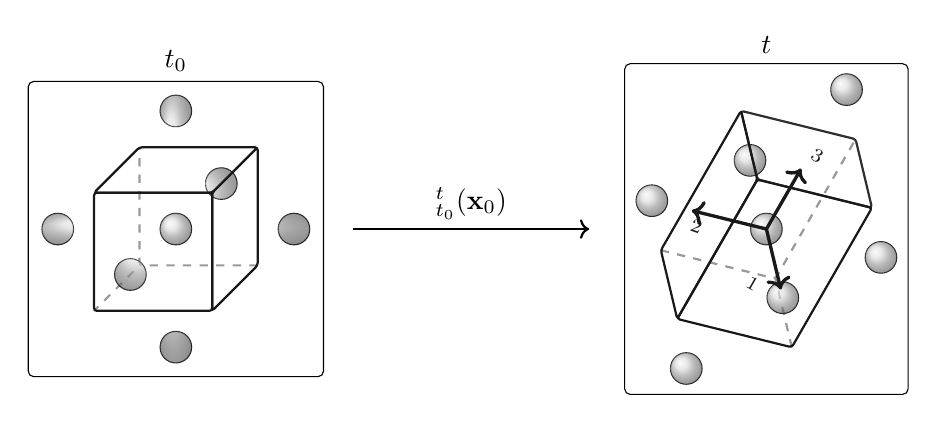
\begin{tikzpicture}

\tdplotsetmaincoords{60}{120}
    %-------------------------------------------------------------------------%
    %                           Initial state                                 %
    %-------------------------------------------------------------------------%
    \coordinate (orig_t0) at (0,0,0);
    % Initial form factors of unit cell
    \pgfmathsetmacro{\sx}{0.75};
    \pgfmathsetmacro{\sy}{0.75};
    \pgfmathsetmacro{\sz}{0.75};

    % Initial separations of fluid elements
    \pgfmathsetmacro{\sepx}{2*\sx};
    \pgfmathsetmacro{\sepy}{2*\sy};
    \pgfmathsetmacro{\sepz}{2*\sz};

    % Radii of fluid elements
    \pgfmathsetmacro{\r}{0.2};

    % Fluid element within unit cell
    \draw[color = black!90] (orig_t0) circle (\r);
    \shade[ball color = gray!40, opacity = 0.6] (orig_t0) circle(\r);


    % Fluid element into the plane
    \draw[color = black!90]  (orig_t0) ++ (0,0,-\sepz) circle (\r);
    \shade[ball color = gray!40, opacity = 0.6] (orig_t0) ++ (0,0,-\sepz) circle(\r);

    % Fluid element to the right
    \draw[color = black!90]  (orig_t0) ++ (\sepx,0,0) circle (\r);
    \shade[ball color = gray!40, opacity = 0.6] (orig_t0) ++ (\sepx,0,0) circle(\r);

    % Fluid element to the left
    \draw[color = black!90]  (orig_t0) ++ (-\sepx,0,0) circle (\r);
    \shade[ball color = gray!40, opacity = 0.6] (orig_t0) ++ (-\sepx,0,0) circle(\r);

    % Fluid element above
    \draw[color = black!90]  (orig_t0) ++ (0,\sepy,0) circle (\r);
    \shade[ball color = gray!40, opacity = 0.6] (orig_t0) ++ (0,\sepy,0) circle(\r);

    % Fluid element below
    \draw[color = black!90]  (orig_t0) ++ (0,-\sepy,0) circle (\r);
    \shade[ball color = gray!40, opacity = 0.6] (orig_t0) ++ (0,-\sepy,0) circle(\r);

    %-------------------------------------------------------------------------%
    % Unit cell
    % Back face
    \path (orig_t0) + (\sx,-\sy,-\sz) coordinate (bbr);
    \path (orig_t0) + (-\sx,-\sy,-\sz) coordinate (bbl);
    \path (orig_t0) + (-\sx,\sy,-\sz) coordinate (btl);
    \draw[thick, dashed, rounded corners = 0.1em, draw opacity = 0.4] (bbr) -- (bbl) -- (btl);
    % Left face
    \path (orig_t0) + (-\sx,-\sy,-\sz) coordinate (lll);
    \path (orig_t0) + (-\sx,-\sy,\sz) coordinate (lul);
    \draw[thick, dashed, shorten >= 0em, shorten <= 0.3em, draw opacity = 0.4] (lll) -- (lul);
    % Front face
    \path (orig_t0) + (\sx,\sy,\sz) coordinate (ftr);
    \path (orig_t0) + (-\sx,\sy,\sz) coordinate (fbr);
    \path (orig_t0) + (-\sx,-\sy,\sz) coordinate (fbl);
    \path (orig_t0) + (\sx,-\sy,\sz) coordinate (ftl);
    \draw[thick, color = black!90, rounded corners = 0.1em] (ftr) -- (fbr) -- (fbl) -- (ftl) -- cycle;
    % Right face
    \path (orig_t0) + (\sx,\sy,\sz) coordinate (rur);
    \path (orig_t0) + (\sx,\sy,-\sz) coordinate (rul);
    \path (orig_t0) + (\sx,-\sy,-\sz) coordinate (rll);
    \path (orig_t0) + (\sx,-\sy,\sz) coordinate (rlr);
    \draw[thick, color = black!90, rounded corners = 0.1em] (rur) -- (rul) -- (rll) -- (rlr) -- cycle;
    % Top face
    \path (orig_t0) + (\sx,\sy,\sz) coordinate (rlr);
    \path (orig_t0) + (-\sx,\sy,\sz) coordinate (llr);
    \path (orig_t0) + (-\sx,\sy,-\sz) coordinate (lur);
    \path (orig_t0) + (\sx,\sy,-\sz) coordinate (rur);
    \draw[thick, color = black!90, rounded corners = 0.1em] (rlr) -- (llr) -- (lur) -- (rur) -- cycle;
    %-------------------------------------------------------------------------%

    % Fluid element out of the plane (drawn in front of the unit cell)
    \draw[color = black!90] (orig_t0) ++ (0,0,\sepz) circle (\r);
    \shade[ball color = gray!30, opacity = 0.6] (orig_t0) ++ (0,0,\sepz) circle(\r);

    % Draw rectangle surrounding the initial state
    \path (orig_t0) + (2.5*\sx, 2.5*\sy, 0) coordinate (ur);
    \path (orig_t0) + (-2.5*\sx, -2.5*\sy, 0) coordinate (ll);
    \path (ur) + (-2.5*\sx,0,0) node[above] {$t_{0}$};
    \draw[thin, rounded corners = 0.2em] (ll) rectangle (ur);

    % Draw arrow connecting initial and final states
    \path (orig_t0) + (3*\sx,0,0) coordinate (l);
    \path (orig_t0) + (7*\sx,0,0) coordinate (r);
    \path (orig_t0) + (5*\sx,0,0) node[above] {$\vct{\phi}_{t_{0}}^{t}(\vct{x}_{0})$};
    \draw[->, thick] (l) -- (r);

    %-------------------------------------------------------------------------%
    %                              Final state                                %
    %-------------------------------------------------------------------------%

    \path (orig_t0) + (10*\sx,0,0) coordinate (orig_t);

    \pgfmathsetmacro{\wou}{0} % Weight one; uno, dos, tres etc
    \pgfmathsetmacro{\wod}{0.72}%{0.6}
    \pgfmathsetmacro{\wot}{0.36}%{0.3}

    \pgfmathsetmacro{\wdu}{0.97}
    \pgfmathsetmacro{\wdd}{-0.24}
    \pgfmathsetmacro{\wdt}{0}

    \pgfmathsetmacro{\wtu}{0.165}
    \pgfmathsetmacro{\wtd}{0.667}
    \pgfmathsetmacro{\wtt}{-1.334}

    % Fluid element within unit cell
    \draw[color = black!90]  (orig_t) circle (\r);
    \shade[ball color = gray!40, opacity = 0.6] (orig_t) circle(\r);

    % Fluid element to the right
    \path (orig_t) + (\wdu*\sepx,\wdd*\sepy,\wdt*\sepz) coordinate (r);
    \draw[color = black!90]  (r) circle (\r);
    \shade[ball color = gray!40, opacity = 0.6] (r) circle(\r);

    % Fluid element to the left
    \path (orig_t) + (-\wdu*\sepx,-\wdd*\sepy,-\wdt*\sepz) coordinate (l);
    \draw[color = black!90]  (l) circle (\r);
    \shade[ball color = gray!40, opacity = 0.6] (l) circle(\r);

    % Fluid element above
    \path (orig_t) + (\wtu*\sepx,\wtd*\sepy,\wtt*\sepz) coordinate (t);
    \draw[color = black!90]  (t) circle (\r);
    \shade[ball color = gray!40, opacity = 0.6] (t) circle(\r);

    % Fluid element below
    \path (orig_t) + (-\wtu*\sepx,-\wtd*\sepy,-\wtt*\sepz) coordinate (b);
    \draw[color = black!90]  (b) circle (\r);
    \shade[ball color = gray!40, opacity = 0.6] (b) circle(\r);

    % Fluid element into the plane
    \path (orig_t) ++ (\wou*\sepx,\wod*\sepy,\wot*\sepz) coordinate (i);
    \draw[color = black!90]  (i) circle (\r);
    \shade[ball color = gray!40, opacity = 0.6] (i) circle(\r);

    % Location of fluid element out of the plane (to be drawn after unit cell)
    \path (orig_t) ++ (-\wou*\sepx,-\wod*\sepy,-\wot*\sepz) coordinate (o);
    %-------------------------------------------------------------------------%
    % Unit cell
    % Back face
    \path ($0.5*(orig_t) + 0.5*(b) + 0.5*(i) - 0.5*(orig_t) - 0.5*(r)+0.5*(orig_t)$) coordinate (bbr);
    \path ($0.5*(orig_t) + 0.5*(b) + 0.5*(i) - 0.5*(orig_t) + 0.5*(r)-0.5*(orig_t)$) coordinate (bbl);
    \path ($0.5*(orig_t) + 0.5*(t) + 0.5*(i) - 0.5*(orig_t) + 0.5*(r)-0.5*(orig_t)$) coordinate (btl);
    \draw[thick, dashed, rounded corners = 0.1em, draw opacity = 0.4] (bbr) -- (bbl) -- (btl);
    % Left face
    \path ($0.5*(orig_t) + 0.5*(l) - 0.5*(i) + 0.5*(orig_t) - 0.5*(b) + 0.5*(orig_t)$) coordinate (lll);
    \path ($0.5*(orig_t) + 0.5*(l) + 0.5*(i) - 0.5*(orig_t) - 0.5*(b) + 0.5*(orig_t)$) coordinate (lul);
    \path ($0.5*(orig_t) + 0.5*(l) + 0.5*(i) - 0.5*(orig_t) + 0.5*(b) - 0.5*(orig_t)$) coordinate (lur);
    \path ($0.5*(orig_t) + 0.5*(l) - 0.5*(i) + 0.5*(orig_t) + 0.5*(b) - 0.5*(orig_t)$) coordinate (llr);
    \draw[thick, color = black!90, rounded corners = 0.1em] (lll) -- (lul) -- (lur) -- (llr) -- cycle;
    % Front face
    \path ($0.5*(orig_t) + 0.5*(o) - 0.5*(l) + 0.5*(orig_t) - 0.5*(b) + 0.5*(orig_t)$) coordinate (ftr);
    \path ($0.5*(orig_t) + 0.5*(o) + 0.5*(l) - 0.5*(orig_t) - 0.5*(b) + 0.5*(orig_t)$) coordinate (fbr);
    \path ($0.5*(orig_t) + 0.5*(o) + 0.5*(l) - 0.5*(orig_t) + 0.5*(b) - 0.5*(orig_t)$) coordinate (fbl);
    \path ($0.5*(orig_t) + 0.5*(o) - 0.5*(l) + 0.5*(orig_t) + 0.5*(b) - 0.5*(orig_t)$) coordinate (ftl);
    \draw[thick, color = black!90, rounded corners = 0.1em] (ftr) -- (fbr) -- (fbl) -- (ftl) -- cycle;
    % Right face
    \path ($0.5*(orig_t) + 0.5*(r) + 0.5*(b) - 0.5*(orig_t) + 0.5*(i) - 0.5*(orig_t)$) coordinate (ril);
    \path ($0.5*(orig_t) + 0.5*(r) + 0.5*(b) - 0.5*(orig_t) - 0.5*(i) + 0.5*(orig_t)$) coordinate (rol);
    \draw[thick, dashed, rounded corners = 0.1em, draw opacity = 0.4] (rol) -- (ril);
    % Top face
    \path ($0.5*(orig_t) + 0.5*(t) - 0.5*(i) + 0.5*(orig_t) - 0.5*(l) + 0.5*(orig_t)$) coordinate (rlr);
    \path ($0.5*(orig_t) + 0.5*(t) + 0.5*(i) - 0.5*(orig_t) - 0.5*(l) + 0.5*(orig_t)$) coordinate (llr);
    \path ($0.5*(orig_t) + 0.5*(t) + 0.5*(i) - 0.5*(orig_t) + 0.5*(l) - 0.5*(orig_t)$) coordinate (lur);
    \path ($0.5*(orig_t) + 0.5*(t) - 0.5*(i) + 0.5*(orig_t) + 0.5*(l) - 0.5*(orig_t)$) coordinate (rur);
    \draw[thick, opacity = 0.9, color = black!90, rounded corners = 0.1em] (rlr) -- (llr) -- (lur) -- (rur) -- cycle;
    %-------------------------------------------------------------------------%
    % Fluid element out of the plane (drawn in front of the unit cell)
    \draw[color = black!90] (o) circle (\r);
    \shade[ball color = gray!40, opacity = 0.6] (o) circle(\r);

    % Draw rectangle surrounding the final state
    \path (orig_t) + (2.4*\sx, 2.8*\sy, 0) coordinate (ur);
    \path (orig_t) + (-2.4*\sx, -2.8*\sy, 0) coordinate (ll);
    \path (ur) + (-2.4*\sx,0,0) node[above] {$t$};
    \draw[thin, rounded corners = 0.2em] (ll) rectangle (ur);

    % Draw strain vectors
    \path ($(orig_t) + 0.88*(o) - 0.88*(orig_t)$) coordinate (onef);
    \draw[->, color = black!90,very thick] (orig_t) -- (onef) node [xshift=-10,yshift=2,rotate=330.11102] {$\vct{\xi}_{1}$};
    \path ($(orig_t) + 0.651*(l) - 0.651*(orig_t)$) coordinate (twof);
    \draw[->, color = black!90,very thick] (orig_t) -- (twof) node [below,xshift=4,rotate=340.11102] {$\vct{\xi}_{2}$};
    \path ($(orig_t) + 0.433*(t) - 0.433*(orig_t)$) coordinate (threef);
    \draw[->, color = black!90,very thick] (orig_t) -- (threef) node [rotate=330.11102,xshift=3,yshift=7] {$\vct{\xi}_{3}$};
\end{tikzpicture}

\end{document}
